\section{Introduction}
% Around a page


% \textit{\blue{1 paragraph about the context and application and its importance.}}

% \textit{\blue{1 paragraph about your specific problem and significance.}}


% \textit{\blue{Add a motivating figure and refer to Fig.~\ref{fig:overview}. Discuss your problem through the scenario illustrated there etc.}}

% \textit{\blue{Discuss why it is novel and why this is not done before too etc.
% }}
% \newpage % remove this one once you have above content



% % figures can be in pdf, or eps format. It is ok to use png, jpeg figures too but others give better quality usually.
% \begin{figure}[t]
% \begin{center}\vspace{-6mm}
% 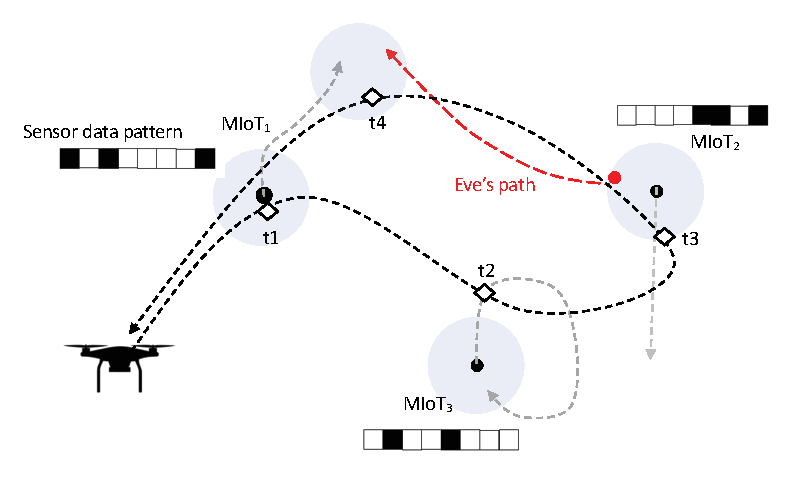
\includegraphics[width=8cm]{Figures/overview.eps}\vspace{0mm}
% \caption{\textit{\blue{Update caption and figure for your project.}} An example scenario with a UAV and three ground
% mobile IoT (MIoT) devices where the UAV needs to travel over the
% area and collect data from each IoT device securely (i.e.,
% while IoT-UAV communication is not eavesdropped) while
% optimizing the delay of the data collected.}\vspace{0mm}
% \label{fig:overview}
% \end{center}
% \end{figure}

% An example scenario is illustrated in Fig.~\ref{fig:overview}, ... 

% \textit{\blue{The last paragraph of Introduction should tell how the rest of the paper is structured. Below is just an example. Feel free to edit.}}

%  The rest of the paper is organized as follows. We discuss the related work in Section~\ref{sec:related}. In Section~\ref{sec:problem}, we provide the system model and provide the problem statement and optimization model. 
% In Section~\ref{sec:results}, we provide simulation/experimental results regarding the performance of proposed solution in various scenarios.
% Finally, we conclude and discuss future work in Section~\ref{sec:conclusion}.

% The rapid urbanization and growth in vehicle ownership have intensified the challenges associated with parking management. Efficient parking space accounting not only alleviates traffic congestion and reduces environmental impact but also improves driver satisfaction. Traditional parking management systems have evolved from manual ticketing to sophisticated sensor-based networks. Most parking decks lacks such systems due to their high cost and intrusive deployment. Recent research has leveraged wireless sensor networks (WSNs) to monitor parking space occupancy, offering a scalable and cost-effective solution for real-time parking guidance\cite{ParkingGuidanceWSN}. In parallel, various studies have demonstrated the utility of wireless sensing modalities, including Bluetooth Low Energy (BLE) and RFID, in detecting vehicle presence and managing parking operations\cite{SmartParkingMDPI, RFIDCloudArxiv}.


% Despite these advances, current approaches typically focus on either enhancing network connectivity using specific sensor technologies or employing wireless sensing for general vehicle detection rather than for precise parking space accounting. For example, BLE-based systems, while effective in communicating occupancy data, often encounter limitations in localization accuracy and robustness under varying environmental conditions\cite{SmartParkingBLE}. Similarly, studies that utilize wireless sensing for multipath analysis have primarily targeted indoor vehicle detection scenarios rather than comprehensive parking space accounting\cite{MultipathRadioSensing}. Moreover, many existing systems involve costly sensor hardware or extensive infrastructure, limiting their practical deployment in resource-constrained urban environments.


% Our research addresses these gaps by proposing a unified, low-cost framework that leverages the strengths of both wireless sensing and WSNs. By integrating these technologies, we aim to achieve higher detection accuracy, improved energy efficiency, and reduced overall system costs—attributes that are critical for large-scale implementations. This work represents a significant advancement over prior systems by unifying wireless sensing with the robust networking capabilities of WSNs, providing a holistic, low-cost approach to parking space accounting in smart city environments.





The rapid urbanization and increase in vehicle ownership have intensified challenges associated with parking management. The average American spends 17 hours per year searching for parking, resulting in an estimated \$73 billion in wasted time and fuel\cite{Inrix}. Efficient detection of empty parking slots not only alleviates traffic congestion and reduces environmental impact but also enhances driver satisfaction as well as increasing the revenue of parking facilities\cite{7895130}. Traditional parking management systems have evolved from manual ticketing to sophisticated sensor-based networks. However, many parking facilities lack such systems due to their high cost and intrusive deployment requirements.




Existing solutions for parking occupancy detection often rely on deploying dedicated sensors in each parking spot, such as magnetic or ultrasonic sensors. While these methods can provide accurate occupancy information, they significantly increase deployment and maintenance costs, making large-scale implementation economically unfeasible\cite{Polycarpou2013SmartPS}. Alternatively, some systems estimate the total number of available parking spaces without identifying the specific locations of empty slots, which limits their practicality for drivers seeking immediate parking.


Wireless sensing has emerged as a promising technology that utilizes existing wireless signals, such as Wi-Fi, to detect and interpret physical phenomena without requiring additional hardware or line-of-sight visibility. By analyzing fine-grained wireless features such as Channel State Information (CSI), wireless sensing enables applications in diverse domains. For instance, it has been used in healthcare to monitor hand movements during physical therapy exercises \cite{10.1145/3688855}, in smart buildings to perform real-time occupancy detection for energy-efficient automation \cite{10.1145/3555776.3577841}, and in activity recognition systems capable of classifying physical gestures and movements \cite{ZHURAVCHAK202259}. These studies demonstrate the versatility and robustness of wireless sensing techniques in dynamic, real-world environments. Our work builds on these principles and adapts them for the problem of detecting empty parking slots in a low-cost, non-intrusive manner.

Recent research has explored the use of wireless sensing techniques for vehicle detection as well. Most of these studies focus moving vehicles, such as those in traffic monitoring \cite{Won2017WiTrafficLA}, rather than stationary vehicles in parking lots. There are few notable studies for parking occupancy detection as well, particularly those leveraging Wi-Fi Channel State Information (CSI). For instance, WiParkFind utilizes off-the-shelf Wi-Fi devices to monitor parking occupancy by analyzing CSI data \cite{8422973}. This approach reduces the need for dedicated sensors and lowers deployment costs. However, WiParkFind focuses on estimating the number of available parking slots without pinpointing their exact locations, which can be less helpful for drivers searching for parking in real-time.

Our research addresses these gaps by proposing a low-cost, non-intrusive system that utilizes wireless sensing techniques and CSI data to accurately detect and identify individual empty parking slots. Unlike existing solutions that either require sensors for each spot or only provide aggregate occupancy counts, our approach leverages CSI-based wireless sensing to pinpoint the exact locations of vacant parking spaces. This easily accesible and deployable solution aims to improve smart parking systems, thereby optimizing urban mobility and parking efficiency.


% % figures can be in pdf, or eps format. It is ok to use png, jpeg figures too but others give better quality usually.
% \begin{figure}[t]
% \begin{center}\vspace{-6mm}
% 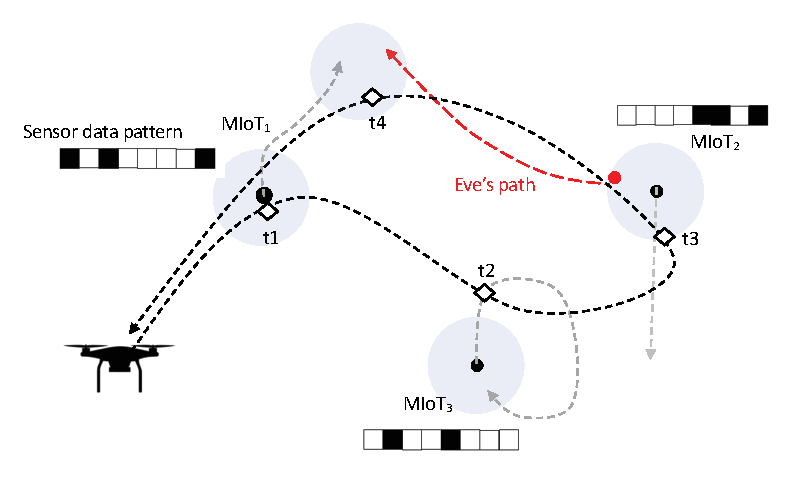
\includegraphics[width=8cm]{Figures/overview.eps}\vspace{0mm}
% \caption{\textit{\blue{Update caption and figure for your project.}} An example scenario with a UAV and three ground
% mobile IoT (MIoT) devices where the UAV needs to travel over the
% area and collect data from each IoT device securely (i.e.,
% while IoT-UAV communication is not eavesdropped) while
% optimizing the delay of the data collected.}\vspace{0mm}
% \label{fig:overview}
% \end{center}
% \end{figure}

% An example scenario is illustrated in Fig.~\ref{fig:overview}, ... 

% \textit{\blue{The last paragraph of Introduction should tell how the rest of the paper is structured. Below is just an example. Feel free to edit.}}

%  The rest of the paper is organized as follows. We discuss the related work in Section~\ref{sec:related}. In Section~\ref{sec:problem}, we provide the system model and provide the problem statement and optimization model. 
% In Section~\ref{sec:results}, we provide simulation/experimental results regarding the performance of proposed solution in various scenarios.
% Finally, we conclude and discuss future work in Section~\ref{sec:conclusion}.






